% Created by tikzDevice version 0.6.2-92-0ad2792 on 2013-03-04 16:57:08
% !TEX encoding = UTF-8 Unicode
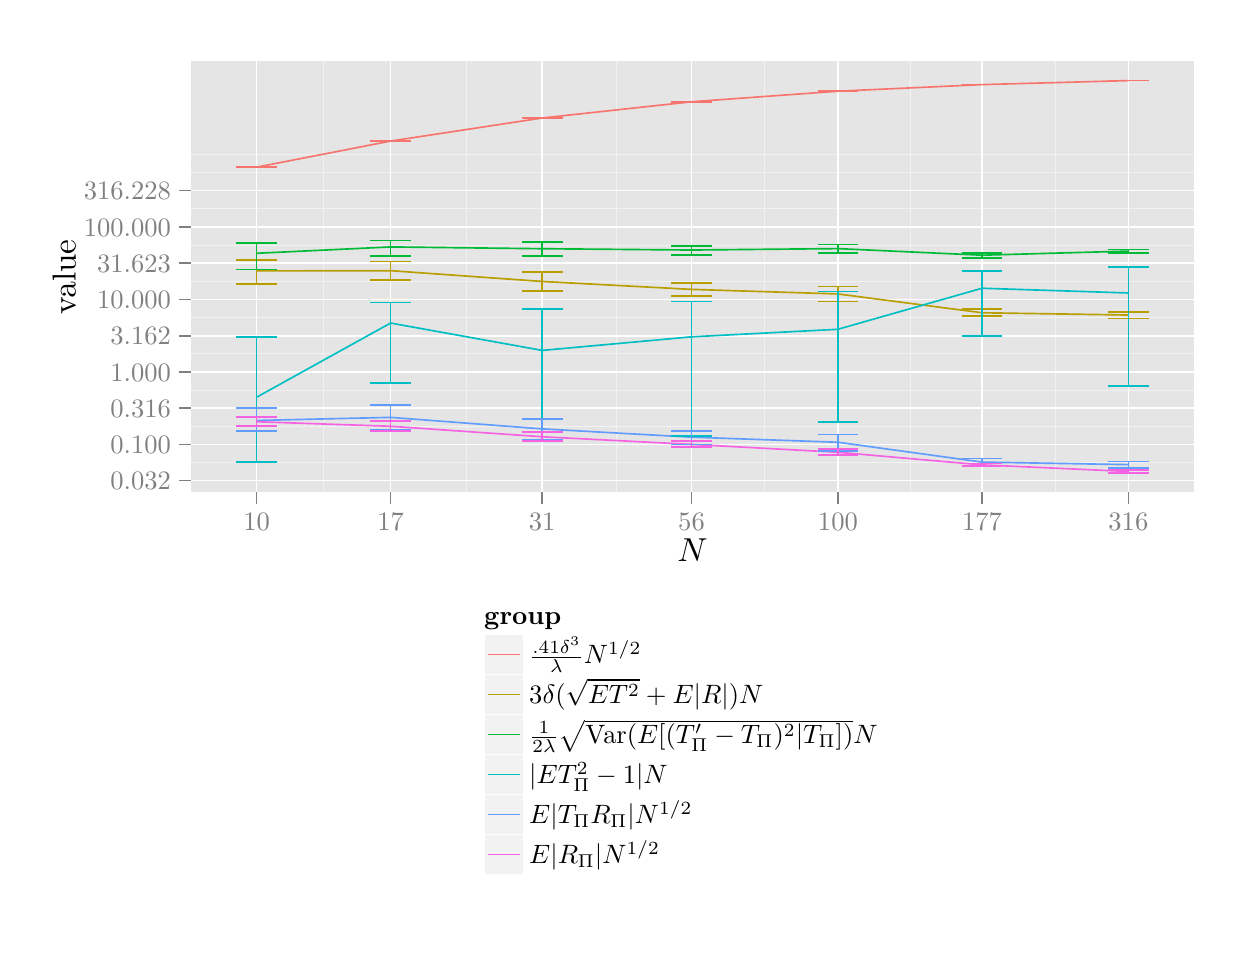
\begin{tikzpicture}[x=1pt,y=1pt]
\definecolor[named]{fillColor}{rgb}{1.00,1.00,1.00}
\path[use as bounding box,fill=fillColor,fill opacity=0.00] (0,0) rectangle (433.62,325.21);
\begin{scope}
\path[clip] (  0.00,  0.00) rectangle (433.62,325.21);
\definecolor[named]{drawColor}{rgb}{1.00,1.00,1.00}
\definecolor[named]{fillColor}{rgb}{1.00,1.00,1.00}

\path[draw=drawColor,line width= 0.6pt,line join=round,line cap=round,fill=fillColor] (  0.00,  0.00) rectangle (433.62,325.21);
\end{scope}
\begin{scope}
\path[clip] ( 58.88,157.27) rectangle (421.57,313.17);
\definecolor[named]{fillColor}{rgb}{0.90,0.90,0.90}

\path[fill=fillColor] ( 58.88,157.27) rectangle (421.57,313.17);
\definecolor[named]{drawColor}{rgb}{0.95,0.95,0.95}

\path[draw=drawColor,line width= 0.3pt,line join=round] ( 58.88,168.09) --
	(421.57,168.09);

\path[draw=drawColor,line width= 0.3pt,line join=round] ( 58.88,181.13) --
	(421.57,181.13);

\path[draw=drawColor,line width= 0.3pt,line join=round] ( 58.88,194.24) --
	(421.57,194.24);

\path[draw=drawColor,line width= 0.3pt,line join=round] ( 58.88,207.35) --
	(421.57,207.35);

\path[draw=drawColor,line width= 0.3pt,line join=round] ( 58.88,220.46) --
	(421.57,220.46);

\path[draw=drawColor,line width= 0.3pt,line join=round] ( 58.88,233.57) --
	(421.57,233.57);

\path[draw=drawColor,line width= 0.3pt,line join=round] ( 58.88,246.68) --
	(421.57,246.68);

\path[draw=drawColor,line width= 0.3pt,line join=round] ( 58.88,259.79) --
	(421.57,259.79);

\path[draw=drawColor,line width= 0.3pt,line join=round] ( 58.88,272.83) --
	(421.57,272.83);

\path[draw=drawColor,line width= 0.3pt,line join=round] ( 58.88,279.31) --
	(421.57,279.31);

\path[draw=drawColor,line width= 0.3pt,line join=round] (106.92,157.27) --
	(106.92,313.17);

\path[draw=drawColor,line width= 0.3pt,line join=round] (158.53,157.27) --
	(158.53,313.17);

\path[draw=drawColor,line width= 0.3pt,line join=round] (212.91,157.27) --
	(212.91,313.17);

\path[draw=drawColor,line width= 0.3pt,line join=round] (266.33,157.27) --
	(266.33,313.17);

\path[draw=drawColor,line width= 0.3pt,line join=round] (318.82,157.27) --
	(318.82,313.17);

\path[draw=drawColor,line width= 0.3pt,line join=round] (371.30,157.27) --
	(371.30,313.17);
\definecolor[named]{drawColor}{rgb}{1.00,1.00,1.00}

\path[draw=drawColor,line width= 0.6pt,line join=round] ( 58.88,161.60) --
	(421.57,161.60);

\path[draw=drawColor,line width= 0.6pt,line join=round] ( 58.88,174.58) --
	(421.57,174.58);

\path[draw=drawColor,line width= 0.6pt,line join=round] ( 58.88,187.68) --
	(421.57,187.68);

\path[draw=drawColor,line width= 0.6pt,line join=round] ( 58.88,200.80) --
	(421.57,200.80);

\path[draw=drawColor,line width= 0.6pt,line join=round] ( 58.88,213.90) --
	(421.57,213.90);

\path[draw=drawColor,line width= 0.6pt,line join=round] ( 58.88,227.01) --
	(421.57,227.01);

\path[draw=drawColor,line width= 0.6pt,line join=round] ( 58.88,240.12) --
	(421.57,240.12);

\path[draw=drawColor,line width= 0.6pt,line join=round] ( 58.88,253.23) --
	(421.57,253.23);

\path[draw=drawColor,line width= 0.6pt,line join=round] ( 58.88,266.34) --
	(421.57,266.34);

\path[draw=drawColor,line width= 0.6pt,line join=round] ( 82.72,157.27) --
	( 82.72,313.17);

\path[draw=drawColor,line width= 0.6pt,line join=round] (131.13,157.27) --
	(131.13,313.17);

\path[draw=drawColor,line width= 0.6pt,line join=round] (185.93,157.27) --
	(185.93,313.17);

\path[draw=drawColor,line width= 0.6pt,line join=round] (239.88,157.27) --
	(239.88,313.17);

\path[draw=drawColor,line width= 0.6pt,line join=round] (292.78,157.27) --
	(292.78,313.17);

\path[draw=drawColor,line width= 0.6pt,line join=round] (344.86,157.27) --
	(344.86,313.17);

\path[draw=drawColor,line width= 0.6pt,line join=round] (397.74,157.27) --
	(397.74,313.17);
\definecolor[named]{drawColor}{rgb}{0.97,0.46,0.43}

\path[draw=drawColor,line width= 0.6pt,line join=round] ( 82.72,274.80) --
	(131.13,284.22) --
	(185.93,292.57) --
	(239.88,298.43) --
	(292.78,302.25) --
	(344.86,304.63) --
	(397.74,306.08);
\definecolor[named]{drawColor}{rgb}{0.72,0.62,0.00}

\path[draw=drawColor,line width= 0.6pt,line join=round] ( 82.72,237.31) --
	(131.13,237.40) --
	(185.93,233.50) --
	(239.88,230.64) --
	(292.78,228.99) --
	(344.86,222.19) --
	(397.74,221.37);
\definecolor[named]{drawColor}{rgb}{0.00,0.73,0.22}

\path[draw=drawColor,line width= 0.6pt,line join=round] ( 82.72,243.68) --
	(131.13,245.98) --
	(185.93,245.33) --
	(239.88,244.86) --
	(292.78,245.37) --
	(344.86,242.99) --
	(397.74,244.47);
\definecolor[named]{drawColor}{rgb}{0.00,0.75,0.77}

\path[draw=drawColor,line width= 0.6pt,line join=round] ( 82.72,191.67) --
	(131.13,218.47) --
	(185.93,208.59) --
	(239.88,213.49) --
	(292.78,216.22) --
	(344.86,231.05) --
	(397.74,229.34);
\definecolor[named]{drawColor}{rgb}{0.38,0.61,1.00}

\path[draw=drawColor,line width= 0.6pt,line join=round] ( 82.72,183.27) --
	(131.13,184.39) --
	(185.93,180.23) --
	(239.88,177.24) --
	(292.78,175.40) --
	(344.86,168.23) --
	(397.74,167.31);
\definecolor[named]{drawColor}{rgb}{0.96,0.39,0.89}

\path[draw=drawColor,line width= 0.6pt,line join=round] ( 82.72,182.81) --
	(131.13,181.18) --
	(185.93,177.38) --
	(239.88,174.63) --
	(292.78,171.78) --
	(344.86,167.22) --
	(397.74,164.84);
\definecolor[named]{drawColor}{rgb}{0.97,0.46,0.43}

\path[draw=drawColor,line width= 0.6pt,line join=round] ( 75.37,274.80) --
	( 90.07,274.80);

\path[draw=drawColor,line width= 0.6pt,line join=round] ( 82.72,274.80) --
	( 82.72,274.80);

\path[draw=drawColor,line width= 0.6pt,line join=round] ( 75.37,274.80) --
	( 90.07,274.80);

\path[draw=drawColor,line width= 0.6pt,line join=round] (123.78,284.22) --
	(138.48,284.22);

\path[draw=drawColor,line width= 0.6pt,line join=round] (131.13,284.22) --
	(131.13,284.22);

\path[draw=drawColor,line width= 0.6pt,line join=round] (123.78,284.22) --
	(138.48,284.22);

\path[draw=drawColor,line width= 0.6pt,line join=round] (178.58,292.57) --
	(193.28,292.57);

\path[draw=drawColor,line width= 0.6pt,line join=round] (185.93,292.57) --
	(185.93,292.57);

\path[draw=drawColor,line width= 0.6pt,line join=round] (178.58,292.57) --
	(193.28,292.57);

\path[draw=drawColor,line width= 0.6pt,line join=round] (232.53,298.43) --
	(247.23,298.43);

\path[draw=drawColor,line width= 0.6pt,line join=round] (239.88,298.43) --
	(239.88,298.43);

\path[draw=drawColor,line width= 0.6pt,line join=round] (232.53,298.43) --
	(247.23,298.43);

\path[draw=drawColor,line width= 0.6pt,line join=round] (285.42,302.25) --
	(300.13,302.25);

\path[draw=drawColor,line width= 0.6pt,line join=round] (292.78,302.25) --
	(292.78,302.25);

\path[draw=drawColor,line width= 0.6pt,line join=round] (285.42,302.25) --
	(300.13,302.25);

\path[draw=drawColor,line width= 0.6pt,line join=round] (337.51,304.63) --
	(352.22,304.63);

\path[draw=drawColor,line width= 0.6pt,line join=round] (344.86,304.63) --
	(344.86,304.63);

\path[draw=drawColor,line width= 0.6pt,line join=round] (337.51,304.63) --
	(352.22,304.63);

\path[draw=drawColor,line width= 0.6pt,line join=round] (390.39,306.08) --
	(405.09,306.08);

\path[draw=drawColor,line width= 0.6pt,line join=round] (397.74,306.08) --
	(397.74,306.08);

\path[draw=drawColor,line width= 0.6pt,line join=round] (390.39,306.08) --
	(405.09,306.08);
\definecolor[named]{drawColor}{rgb}{0.72,0.62,0.00}

\path[draw=drawColor,line width= 0.6pt,line join=round] ( 75.37,241.36) --
	( 90.07,241.36);

\path[draw=drawColor,line width= 0.6pt,line join=round] ( 82.72,241.36) --
	( 82.72,232.58);

\path[draw=drawColor,line width= 0.6pt,line join=round] ( 75.37,232.58) --
	( 90.07,232.58);

\path[draw=drawColor,line width= 0.6pt,line join=round] (123.78,240.74) --
	(138.48,240.74);

\path[draw=drawColor,line width= 0.6pt,line join=round] (131.13,240.74) --
	(131.13,233.93);

\path[draw=drawColor,line width= 0.6pt,line join=round] (123.78,233.93) --
	(138.48,233.93);

\path[draw=drawColor,line width= 0.6pt,line join=round] (178.58,236.92) --
	(193.28,236.92);

\path[draw=drawColor,line width= 0.6pt,line join=round] (185.93,236.92) --
	(185.93,230.03);

\path[draw=drawColor,line width= 0.6pt,line join=round] (178.58,230.03) --
	(193.28,230.03);

\path[draw=drawColor,line width= 0.6pt,line join=round] (232.53,232.93) --
	(247.23,232.93);

\path[draw=drawColor,line width= 0.6pt,line join=round] (239.88,232.93) --
	(239.88,228.14);

\path[draw=drawColor,line width= 0.6pt,line join=round] (232.53,228.14) --
	(247.23,228.14);

\path[draw=drawColor,line width= 0.6pt,line join=round] (285.42,231.63) --
	(300.13,231.63);

\path[draw=drawColor,line width= 0.6pt,line join=round] (292.78,231.63) --
	(292.78,226.28);

\path[draw=drawColor,line width= 0.6pt,line join=round] (285.42,226.28) --
	(300.13,226.28);

\path[draw=drawColor,line width= 0.6pt,line join=round] (337.51,223.51) --
	(352.22,223.51);

\path[draw=drawColor,line width= 0.6pt,line join=round] (344.86,223.51) --
	(344.86,221.00);

\path[draw=drawColor,line width= 0.6pt,line join=round] (337.51,221.00) --
	(352.22,221.00);

\path[draw=drawColor,line width= 0.6pt,line join=round] (390.39,222.55) --
	(405.09,222.55);

\path[draw=drawColor,line width= 0.6pt,line join=round] (397.74,222.55) --
	(397.74,220.15);

\path[draw=drawColor,line width= 0.6pt,line join=round] (390.39,220.15) --
	(405.09,220.15);
\definecolor[named]{drawColor}{rgb}{0.00,0.73,0.22}

\path[draw=drawColor,line width= 0.6pt,line join=round] ( 75.37,247.35) --
	( 90.07,247.35);

\path[draw=drawColor,line width= 0.6pt,line join=round] ( 82.72,247.35) --
	( 82.72,237.83);

\path[draw=drawColor,line width= 0.6pt,line join=round] ( 75.37,237.83) --
	( 90.07,237.83);

\path[draw=drawColor,line width= 0.6pt,line join=round] (123.78,248.29) --
	(138.48,248.29);

\path[draw=drawColor,line width= 0.6pt,line join=round] (131.13,248.29) --
	(131.13,242.71);

\path[draw=drawColor,line width= 0.6pt,line join=round] (123.78,242.71) --
	(138.48,242.71);

\path[draw=drawColor,line width= 0.6pt,line join=round] (178.58,247.75) --
	(193.28,247.75);

\path[draw=drawColor,line width= 0.6pt,line join=round] (185.93,247.75) --
	(185.93,242.69);

\path[draw=drawColor,line width= 0.6pt,line join=round] (178.58,242.69) --
	(193.28,242.69);

\path[draw=drawColor,line width= 0.6pt,line join=round] (232.53,246.33) --
	(247.23,246.33);

\path[draw=drawColor,line width= 0.6pt,line join=round] (239.88,246.33) --
	(239.88,243.15);

\path[draw=drawColor,line width= 0.6pt,line join=round] (232.53,243.15) --
	(247.23,243.15);

\path[draw=drawColor,line width= 0.6pt,line join=round] (285.42,246.86) --
	(300.13,246.86);

\path[draw=drawColor,line width= 0.6pt,line join=round] (292.78,246.86) --
	(292.78,243.71);

\path[draw=drawColor,line width= 0.6pt,line join=round] (285.42,243.71) --
	(300.13,243.71);

\path[draw=drawColor,line width= 0.6pt,line join=round] (337.51,243.82) --
	(352.22,243.82);

\path[draw=drawColor,line width= 0.6pt,line join=round] (344.86,243.82) --
	(344.86,242.07);

\path[draw=drawColor,line width= 0.6pt,line join=round] (337.51,242.07) --
	(352.22,242.07);

\path[draw=drawColor,line width= 0.6pt,line join=round] (390.39,245.11) --
	(405.09,245.11);

\path[draw=drawColor,line width= 0.6pt,line join=round] (397.74,245.11) --
	(397.74,243.71);

\path[draw=drawColor,line width= 0.6pt,line join=round] (390.39,243.71) --
	(405.09,243.71);
\definecolor[named]{drawColor}{rgb}{0.00,0.75,0.77}

\path[draw=drawColor,line width= 0.6pt,line join=round] ( 75.37,213.48) --
	( 90.07,213.48);

\path[draw=drawColor,line width= 0.6pt,line join=round] ( 82.72,213.48) --
	( 82.72,168.23);

\path[draw=drawColor,line width= 0.6pt,line join=round] ( 75.37,168.23) --
	( 90.07,168.23);

\path[draw=drawColor,line width= 0.6pt,line join=round] (123.78,225.93) --
	(138.48,225.93);

\path[draw=drawColor,line width= 0.6pt,line join=round] (131.13,225.93) --
	(131.13,196.83);

\path[draw=drawColor,line width= 0.6pt,line join=round] (123.78,196.83) --
	(138.48,196.83);

\path[draw=drawColor,line width= 0.6pt,line join=round] (178.58,223.47) --
	(193.28,223.47);

\path[draw=drawColor,line width= 0.6pt,line join=round] (185.93,223.47) --
	(185.93,176.24);

\path[draw=drawColor,line width= 0.6pt,line join=round] (178.58,176.24) --
	(193.28,176.24);

\path[draw=drawColor,line width= 0.6pt,line join=round] (232.53,226.30) --
	(247.23,226.30);

\path[draw=drawColor,line width= 0.6pt,line join=round] (239.88,226.30) --
	(239.88,177.54);

\path[draw=drawColor,line width= 0.6pt,line join=round] (232.53,177.54) --
	(247.23,177.54);

\path[draw=drawColor,line width= 0.6pt,line join=round] (285.42,229.84) --
	(300.13,229.84);

\path[draw=drawColor,line width= 0.6pt,line join=round] (292.78,229.84) --
	(292.78,182.82);

\path[draw=drawColor,line width= 0.6pt,line join=round] (285.42,182.82) --
	(300.13,182.82);

\path[draw=drawColor,line width= 0.6pt,line join=round] (337.51,237.29) --
	(352.22,237.29);

\path[draw=drawColor,line width= 0.6pt,line join=round] (344.86,237.29) --
	(344.86,213.80);

\path[draw=drawColor,line width= 0.6pt,line join=round] (337.51,213.80) --
	(352.22,213.80);

\path[draw=drawColor,line width= 0.6pt,line join=round] (390.39,238.74) --
	(405.09,238.74);

\path[draw=drawColor,line width= 0.6pt,line join=round] (397.74,238.74) --
	(397.74,195.69);

\path[draw=drawColor,line width= 0.6pt,line join=round] (390.39,195.69) --
	(405.09,195.69);
\definecolor[named]{drawColor}{rgb}{0.38,0.61,1.00}

\path[draw=drawColor,line width= 0.6pt,line join=round] ( 75.37,187.72) --
	( 90.07,187.72);

\path[draw=drawColor,line width= 0.6pt,line join=round] ( 82.72,187.72) --
	( 82.72,179.35);

\path[draw=drawColor,line width= 0.6pt,line join=round] ( 75.37,179.35) --
	( 90.07,179.35);

\path[draw=drawColor,line width= 0.6pt,line join=round] (123.78,188.92) --
	(138.48,188.92);

\path[draw=drawColor,line width= 0.6pt,line join=round] (131.13,188.92) --
	(131.13,179.87);

\path[draw=drawColor,line width= 0.6pt,line join=round] (123.78,179.87) --
	(138.48,179.87);

\path[draw=drawColor,line width= 0.6pt,line join=round] (178.58,183.83) --
	(193.28,183.83);

\path[draw=drawColor,line width= 0.6pt,line join=round] (185.93,183.83) --
	(185.93,176.32);

\path[draw=drawColor,line width= 0.6pt,line join=round] (178.58,176.32) --
	(193.28,176.32);

\path[draw=drawColor,line width= 0.6pt,line join=round] (232.53,179.58) --
	(247.23,179.58);

\path[draw=drawColor,line width= 0.6pt,line join=round] (239.88,179.58) --
	(239.88,174.64);

\path[draw=drawColor,line width= 0.6pt,line join=round] (232.53,174.64) --
	(247.23,174.64);

\path[draw=drawColor,line width= 0.6pt,line join=round] (285.42,178.23) --
	(300.13,178.23);

\path[draw=drawColor,line width= 0.6pt,line join=round] (292.78,178.23) --
	(292.78,172.23);

\path[draw=drawColor,line width= 0.6pt,line join=round] (285.42,172.23) --
	(300.13,172.23);

\path[draw=drawColor,line width= 0.6pt,line join=round] (337.51,169.49) --
	(352.22,169.49);

\path[draw=drawColor,line width= 0.6pt,line join=round] (344.86,169.49) --
	(344.86,166.82);

\path[draw=drawColor,line width= 0.6pt,line join=round] (337.51,166.82) --
	(352.22,166.82);

\path[draw=drawColor,line width= 0.6pt,line join=round] (390.39,168.50) --
	(405.09,168.50);

\path[draw=drawColor,line width= 0.6pt,line join=round] (397.74,168.50) --
	(397.74,166.07);

\path[draw=drawColor,line width= 0.6pt,line join=round] (390.39,166.07) --
	(405.09,166.07);
\definecolor[named]{drawColor}{rgb}{0.96,0.39,0.89}

\path[draw=drawColor,line width= 0.6pt,line join=round] ( 75.37,184.55) --
	( 90.07,184.55);

\path[draw=drawColor,line width= 0.6pt,line join=round] ( 82.72,184.55) --
	( 82.72,181.26);

\path[draw=drawColor,line width= 0.6pt,line join=round] ( 75.37,181.26) --
	( 90.07,181.26);

\path[draw=drawColor,line width= 0.6pt,line join=round] (123.78,183.06) --
	(138.48,183.06);

\path[draw=drawColor,line width= 0.6pt,line join=round] (131.13,183.06) --
	(131.13,179.43);

\path[draw=drawColor,line width= 0.6pt,line join=round] (123.78,179.43) --
	(138.48,179.43);

\path[draw=drawColor,line width= 0.6pt,line join=round] (178.58,179.19) --
	(193.28,179.19);

\path[draw=drawColor,line width= 0.6pt,line join=round] (185.93,179.19) --
	(185.93,175.79);

\path[draw=drawColor,line width= 0.6pt,line join=round] (178.58,175.79) --
	(193.28,175.79);

\path[draw=drawColor,line width= 0.6pt,line join=round] (232.53,175.77) --
	(247.23,175.77);

\path[draw=drawColor,line width= 0.6pt,line join=round] (239.88,175.77) --
	(239.88,173.57);

\path[draw=drawColor,line width= 0.6pt,line join=round] (232.53,173.57) --
	(247.23,173.57);

\path[draw=drawColor,line width= 0.6pt,line join=round] (285.42,172.94) --
	(300.13,172.94);

\path[draw=drawColor,line width= 0.6pt,line join=round] (292.78,172.94) --
	(292.78,170.74);

\path[draw=drawColor,line width= 0.6pt,line join=round] (285.42,170.74) --
	(300.13,170.74);

\path[draw=drawColor,line width= 0.6pt,line join=round] (337.51,167.75) --
	(352.22,167.75);

\path[draw=drawColor,line width= 0.6pt,line join=round] (344.86,167.75) --
	(344.86,166.71);

\path[draw=drawColor,line width= 0.6pt,line join=round] (337.51,166.71) --
	(352.22,166.71);

\path[draw=drawColor,line width= 0.6pt,line join=round] (390.39,165.34) --
	(405.09,165.34);

\path[draw=drawColor,line width= 0.6pt,line join=round] (397.74,165.34) --
	(397.74,164.35);

\path[draw=drawColor,line width= 0.6pt,line join=round] (390.39,164.35) --
	(405.09,164.35);
\end{scope}
\begin{scope}
\path[clip] (  0.00,  0.00) rectangle (433.62,325.21);
\definecolor[named]{drawColor}{rgb}{0.50,0.50,0.50}

\node[text=drawColor,anchor=base east,inner sep=0pt, outer sep=0pt, scale=  0.96] at ( 51.77,158.30) {0.032};

\node[text=drawColor,anchor=base east,inner sep=0pt, outer sep=0pt, scale=  0.96] at ( 51.77,171.27) {0.100};

\node[text=drawColor,anchor=base east,inner sep=0pt, outer sep=0pt, scale=  0.96] at ( 51.77,184.37) {0.316};

\node[text=drawColor,anchor=base east,inner sep=0pt, outer sep=0pt, scale=  0.96] at ( 51.77,197.49) {1.000};

\node[text=drawColor,anchor=base east,inner sep=0pt, outer sep=0pt, scale=  0.96] at ( 51.77,210.60) {3.162};

\node[text=drawColor,anchor=base east,inner sep=0pt, outer sep=0pt, scale=  0.96] at ( 51.77,223.71) {10.000};

\node[text=drawColor,anchor=base east,inner sep=0pt, outer sep=0pt, scale=  0.96] at ( 51.77,236.82) {31.623};

\node[text=drawColor,anchor=base east,inner sep=0pt, outer sep=0pt, scale=  0.96] at ( 51.77,249.93) {100.000};

\node[text=drawColor,anchor=base east,inner sep=0pt, outer sep=0pt, scale=  0.96] at ( 51.77,263.03) {316.228};
\end{scope}
\begin{scope}
\path[clip] (  0.00,  0.00) rectangle (433.62,325.21);
\definecolor[named]{drawColor}{rgb}{0.50,0.50,0.50}

\path[draw=drawColor,line width= 0.6pt,line join=round] ( 54.61,161.60) --
	( 58.88,161.60);

\path[draw=drawColor,line width= 0.6pt,line join=round] ( 54.61,174.58) --
	( 58.88,174.58);

\path[draw=drawColor,line width= 0.6pt,line join=round] ( 54.61,187.68) --
	( 58.88,187.68);

\path[draw=drawColor,line width= 0.6pt,line join=round] ( 54.61,200.80) --
	( 58.88,200.80);

\path[draw=drawColor,line width= 0.6pt,line join=round] ( 54.61,213.90) --
	( 58.88,213.90);

\path[draw=drawColor,line width= 0.6pt,line join=round] ( 54.61,227.01) --
	( 58.88,227.01);

\path[draw=drawColor,line width= 0.6pt,line join=round] ( 54.61,240.12) --
	( 58.88,240.12);

\path[draw=drawColor,line width= 0.6pt,line join=round] ( 54.61,253.23) --
	( 58.88,253.23);

\path[draw=drawColor,line width= 0.6pt,line join=round] ( 54.61,266.34) --
	( 58.88,266.34);
\end{scope}
\begin{scope}
\path[clip] (  0.00,  0.00) rectangle (433.62,325.21);
\definecolor[named]{drawColor}{rgb}{0.50,0.50,0.50}

\path[draw=drawColor,line width= 0.6pt,line join=round] ( 82.72,153.00) --
	( 82.72,157.27);

\path[draw=drawColor,line width= 0.6pt,line join=round] (131.13,153.00) --
	(131.13,157.27);

\path[draw=drawColor,line width= 0.6pt,line join=round] (185.93,153.00) --
	(185.93,157.27);

\path[draw=drawColor,line width= 0.6pt,line join=round] (239.88,153.00) --
	(239.88,157.27);

\path[draw=drawColor,line width= 0.6pt,line join=round] (292.78,153.00) --
	(292.78,157.27);

\path[draw=drawColor,line width= 0.6pt,line join=round] (344.86,153.00) --
	(344.86,157.27);

\path[draw=drawColor,line width= 0.6pt,line join=round] (397.74,153.00) --
	(397.74,157.27);
\end{scope}
\begin{scope}
\path[clip] (  0.00,  0.00) rectangle (433.62,325.21);
\definecolor[named]{drawColor}{rgb}{0.50,0.50,0.50}

\node[text=drawColor,anchor=base,inner sep=0pt, outer sep=0pt, scale=  0.96] at ( 82.72,143.54) {10};

\node[text=drawColor,anchor=base,inner sep=0pt, outer sep=0pt, scale=  0.96] at (131.13,143.54) {17};

\node[text=drawColor,anchor=base,inner sep=0pt, outer sep=0pt, scale=  0.96] at (185.93,143.54) {31};

\node[text=drawColor,anchor=base,inner sep=0pt, outer sep=0pt, scale=  0.96] at (239.88,143.54) {56};

\node[text=drawColor,anchor=base,inner sep=0pt, outer sep=0pt, scale=  0.96] at (292.78,143.54) {100};

\node[text=drawColor,anchor=base,inner sep=0pt, outer sep=0pt, scale=  0.96] at (344.86,143.54) {177};

\node[text=drawColor,anchor=base,inner sep=0pt, outer sep=0pt, scale=  0.96] at (397.74,143.54) {316};
\end{scope}
\begin{scope}
\path[clip] (  0.00,  0.00) rectangle (433.62,325.21);
\definecolor[named]{drawColor}{rgb}{0.00,0.00,0.00}

\node[text=drawColor,anchor=base,inner sep=0pt, outer sep=0pt, scale=  1.20] at (240.23,132.27) {$N$};
\end{scope}
\begin{scope}
\path[clip] (  0.00,  0.00) rectangle (433.62,325.21);
\definecolor[named]{drawColor}{rgb}{0.00,0.00,0.00}

\node[text=drawColor,rotate= 90.00,anchor=base,inner sep=0pt, outer sep=0pt, scale=  1.20] at ( 17.30,235.22) {value};
\end{scope}
\begin{scope}
\path[clip] (  0.00,  0.00) rectangle (433.62,325.21);
\definecolor[named]{fillColor}{rgb}{1.00,1.00,1.00}

\path[fill=fillColor] (160.71, 14.89) rectangle (319.75,120.39);
\end{scope}
\begin{scope}
\path[clip] (  0.00,  0.00) rectangle (433.62,325.21);
\definecolor[named]{drawColor}{rgb}{0.00,0.00,0.00}

\node[text=drawColor,anchor=base west,inner sep=0pt, outer sep=0pt, scale=  0.96] at (164.98,109.50) {\bfseries group};
\end{scope}
\begin{scope}
\path[clip] (  0.00,  0.00) rectangle (433.62,325.21);
\definecolor[named]{drawColor}{rgb}{1.00,1.00,1.00}
\definecolor[named]{fillColor}{rgb}{0.95,0.95,0.95}

\path[draw=drawColor,line width= 0.6pt,line join=round,line cap=round,fill=fillColor] (164.98, 91.43) rectangle (179.43,105.88);
\end{scope}
\begin{scope}
\path[clip] (  0.00,  0.00) rectangle (433.62,325.21);
\definecolor[named]{drawColor}{rgb}{0.97,0.46,0.43}

\path[draw=drawColor,line width= 0.6pt,line join=round] (166.42, 98.66) -- (177.98, 98.66);
\end{scope}
\begin{scope}
\path[clip] (  0.00,  0.00) rectangle (433.62,325.21);
\definecolor[named]{drawColor}{rgb}{0.97,0.46,0.43}

\path[draw=drawColor,line width= 0.6pt,line join=round] (166.42, 98.66) -- (177.98, 98.66);
\end{scope}
\begin{scope}
\path[clip] (  0.00,  0.00) rectangle (433.62,325.21);
\definecolor[named]{drawColor}{rgb}{1.00,1.00,1.00}
\definecolor[named]{fillColor}{rgb}{0.95,0.95,0.95}

\path[draw=drawColor,line width= 0.6pt,line join=round,line cap=round,fill=fillColor] (164.98, 76.97) rectangle (179.43, 91.43);
\end{scope}
\begin{scope}
\path[clip] (  0.00,  0.00) rectangle (433.62,325.21);
\definecolor[named]{drawColor}{rgb}{0.72,0.62,0.00}

\path[draw=drawColor,line width= 0.6pt,line join=round] (166.42, 84.20) -- (177.98, 84.20);
\end{scope}
\begin{scope}
\path[clip] (  0.00,  0.00) rectangle (433.62,325.21);
\definecolor[named]{drawColor}{rgb}{0.72,0.62,0.00}

\path[draw=drawColor,line width= 0.6pt,line join=round] (166.42, 84.20) -- (177.98, 84.20);
\end{scope}
\begin{scope}
\path[clip] (  0.00,  0.00) rectangle (433.62,325.21);
\definecolor[named]{drawColor}{rgb}{1.00,1.00,1.00}
\definecolor[named]{fillColor}{rgb}{0.95,0.95,0.95}

\path[draw=drawColor,line width= 0.6pt,line join=round,line cap=round,fill=fillColor] (164.98, 62.52) rectangle (179.43, 76.97);
\end{scope}
\begin{scope}
\path[clip] (  0.00,  0.00) rectangle (433.62,325.21);
\definecolor[named]{drawColor}{rgb}{0.00,0.73,0.22}

\path[draw=drawColor,line width= 0.6pt,line join=round] (166.42, 69.75) -- (177.98, 69.75);
\end{scope}
\begin{scope}
\path[clip] (  0.00,  0.00) rectangle (433.62,325.21);
\definecolor[named]{drawColor}{rgb}{0.00,0.73,0.22}

\path[draw=drawColor,line width= 0.6pt,line join=round] (166.42, 69.75) -- (177.98, 69.75);
\end{scope}
\begin{scope}
\path[clip] (  0.00,  0.00) rectangle (433.62,325.21);
\definecolor[named]{drawColor}{rgb}{1.00,1.00,1.00}
\definecolor[named]{fillColor}{rgb}{0.95,0.95,0.95}

\path[draw=drawColor,line width= 0.6pt,line join=round,line cap=round,fill=fillColor] (164.98, 48.07) rectangle (179.43, 62.52);
\end{scope}
\begin{scope}
\path[clip] (  0.00,  0.00) rectangle (433.62,325.21);
\definecolor[named]{drawColor}{rgb}{0.00,0.75,0.77}

\path[draw=drawColor,line width= 0.6pt,line join=round] (166.42, 55.29) -- (177.98, 55.29);
\end{scope}
\begin{scope}
\path[clip] (  0.00,  0.00) rectangle (433.62,325.21);
\definecolor[named]{drawColor}{rgb}{0.00,0.75,0.77}

\path[draw=drawColor,line width= 0.6pt,line join=round] (166.42, 55.29) -- (177.98, 55.29);
\end{scope}
\begin{scope}
\path[clip] (  0.00,  0.00) rectangle (433.62,325.21);
\definecolor[named]{drawColor}{rgb}{1.00,1.00,1.00}
\definecolor[named]{fillColor}{rgb}{0.95,0.95,0.95}

\path[draw=drawColor,line width= 0.6pt,line join=round,line cap=round,fill=fillColor] (164.98, 33.61) rectangle (179.43, 48.07);
\end{scope}
\begin{scope}
\path[clip] (  0.00,  0.00) rectangle (433.62,325.21);
\definecolor[named]{drawColor}{rgb}{0.38,0.61,1.00}

\path[draw=drawColor,line width= 0.6pt,line join=round] (166.42, 40.84) -- (177.98, 40.84);
\end{scope}
\begin{scope}
\path[clip] (  0.00,  0.00) rectangle (433.62,325.21);
\definecolor[named]{drawColor}{rgb}{0.38,0.61,1.00}

\path[draw=drawColor,line width= 0.6pt,line join=round] (166.42, 40.84) -- (177.98, 40.84);
\end{scope}
\begin{scope}
\path[clip] (  0.00,  0.00) rectangle (433.62,325.21);
\definecolor[named]{drawColor}{rgb}{1.00,1.00,1.00}
\definecolor[named]{fillColor}{rgb}{0.95,0.95,0.95}

\path[draw=drawColor,line width= 0.6pt,line join=round,line cap=round,fill=fillColor] (164.98, 19.16) rectangle (179.43, 33.61);
\end{scope}
\begin{scope}
\path[clip] (  0.00,  0.00) rectangle (433.62,325.21);
\definecolor[named]{drawColor}{rgb}{0.96,0.39,0.89}

\path[draw=drawColor,line width= 0.6pt,line join=round] (166.42, 26.39) -- (177.98, 26.39);
\end{scope}
\begin{scope}
\path[clip] (  0.00,  0.00) rectangle (433.62,325.21);
\definecolor[named]{drawColor}{rgb}{0.96,0.39,0.89}

\path[draw=drawColor,line width= 0.6pt,line join=round] (166.42, 26.39) -- (177.98, 26.39);
\end{scope}
\begin{scope}
\path[clip] (  0.00,  0.00) rectangle (433.62,325.21);
\definecolor[named]{drawColor}{rgb}{0.00,0.00,0.00}

\node[text=drawColor,anchor=base west,inner sep=0pt, outer sep=0pt, scale=  0.96] at (181.24, 95.35) {$\frac{.41\delta^3}{\lambda}N^{1/2}\quad $};
\end{scope}
\begin{scope}
\path[clip] (  0.00,  0.00) rectangle (433.62,325.21);
\definecolor[named]{drawColor}{rgb}{0.00,0.00,0.00}

\node[text=drawColor,anchor=base west,inner sep=0pt, outer sep=0pt, scale=  0.96] at (181.24, 80.90) {$3\delta(\sqrt{\mathbb{E}T^2}+\mathbb{E}|R|)N\quad $};
\end{scope}
\begin{scope}
\path[clip] (  0.00,  0.00) rectangle (433.62,325.21);
\definecolor[named]{drawColor}{rgb}{0.00,0.00,0.00}

\node[text=drawColor,anchor=base west,inner sep=0pt, outer sep=0pt, scale=  0.96] at (181.24, 66.44) {$\frac{1}{2\lambda}\sqrt{\mathrm{Var}(\mathbb{E}[(T'_{\Pi}-T_{\Pi})^2|T_{\Pi}])}N\quad $};
\end{scope}
\begin{scope}
\path[clip] (  0.00,  0.00) rectangle (433.62,325.21);
\definecolor[named]{drawColor}{rgb}{0.00,0.00,0.00}

\node[text=drawColor,anchor=base west,inner sep=0pt, outer sep=0pt, scale=  0.96] at (181.24, 51.99) {$|\mathbb{E}T_{\Pi}^2-1|N\quad $};
\end{scope}
\begin{scope}
\path[clip] (  0.00,  0.00) rectangle (433.62,325.21);
\definecolor[named]{drawColor}{rgb}{0.00,0.00,0.00}

\node[text=drawColor,anchor=base west,inner sep=0pt, outer sep=0pt, scale=  0.96] at (181.24, 37.53) {$\mathbb{E}|T_{\Pi}R_{\Pi}|N^{1/2}\quad $};
\end{scope}
\begin{scope}
\path[clip] (  0.00,  0.00) rectangle (433.62,325.21);
\definecolor[named]{drawColor}{rgb}{0.00,0.00,0.00}

\node[text=drawColor,anchor=base west,inner sep=0pt, outer sep=0pt, scale=  0.96] at (181.24, 23.08) {$\mathbb{E}|R_{\Pi}|N^{1/2}\quad $};
\end{scope}
\end{tikzpicture}
